% 1. Introducción a la teoría de códigos lineales. 
% Aquí cuanto más quieras leer del libro de Huffman y Pless, mejor. 
% Necesario sólo es el capítulo 1 y el 3 (no todo del 3). 
% Y, aunque no los utilicemos, puedes leerte el capítulo de códigos cíclicos. 
% Es importante centrarse en lo que es la distancia, y que es un problema NP-completo (archivo VARDY.pdf)) ya que es lo que le da seguridad a los criptosistemas.

\chapter{Introducción a la teoría de códigos lineales}

En este capítulo  introduciremos los conceptos y resultados fundamentales sobre la teoría de códigos lineales. Empezaremos con la definiendo básica de código para estudiar posteriormente el concepto de código lineal y algunas de sus propiedades más relevante, junto con otros conceptos relacionados. Finalmente, introduciremos el algoritmo de Brouwer-Zimmermann, que permite calcular un concepto muy importante en la teoría de códigos. 

El desarrollo de este capítulo se ha basado, principalmente, en \cite[Capítulo 1]{Huffman_Pless_2010}.

\section{Introducción}

Supongamos que queremos enviar un mensaje, por lo que habrá un emisor y un receptor que se comunican, en general, en una dirección. Este mensaje es una secuencia finita de elementos de un alfabeto dado y es enviado por un \emph{canal de comunicación}, a través del cual es posible que la información se altere por las interferencias y el ruido, lo que se conoce como \emph{ruido del canal}. Es por esto que hay que hacer una \emph{traducción} entre el mensaje original (o \emph{palabra fuente}) $x$ y el tipo de mensaje $c$ que el canal está capacitado para enviar (\emph{palabras código}). Esta manipulación consiste en proteger el mensaje original, ya sea por ejemplo añadiendo redundancia o repitiéndolo, para que posteriormente se pueda corregir el ruido hasta cierto punto. Este proceso se llama \emph{codificación}. Una vez codificado el mensaje, lo enviamos a través del canal, y nuestro intermediario (el receptor) recibe un mensaje codificado (\emph{palabra recibida}) posiblemente erróneo. Una vez recibido, empieza el proceso llamado \emph{corrección de errores}, que consiste en recuperar el mensaje original corrigiendo los errores que se hubieran producido. El mensaje recibido $c'$ es traducido nuevamente a términos originales $x'$, es decir, es \emph{decodificado}. La siguiente figura representa un esquema de este proceso.

\begin{figure}[H]
	\center
	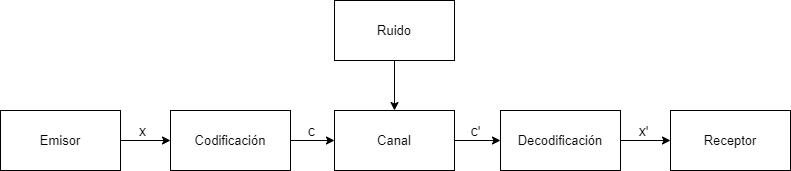
\includegraphics[scale=0.5]{figures/Diagrama_comunicacion.png}
	\caption{Esquema del modelo de comunicación, \cite{Podesta_2006}.}
\end{figure}

Las flechas indican que la comunicación es en un solo sentido.

En general, $x' \neq x$ y es deseable que este error sea detectado (lo cual permite pedir una retransmisión del mensaje) y en lo posible corregido.

La \emph{Teoría de Códigos Autocorrectores} se ocupa del segundo y cuarto pasos del esquema anterior, es decir, de la codificación y decodificación de mensajes, junto con el problema de detectar y corregir errores. A veces no es posible pedir retransmisión de mensajes y es por eso que los códigos autocorrectores son tan útiles y necesarios.

La calidad de un código con mensajes de longitud $k$ y palabras código de longitud $n$ vendrá dada por las siguientes características.

\begin{itemize}
    \item El cociente $\frac{k}{n}$, el \emph{ratio de información} del código, que mide el esfuerzo necesario para transmitir un mensaje codificado.
    \item La \emph{distancia mínima relativa} $d$ que es aproximadamente el doble de la proporción de errores que se pueden corregir en cada mensaje codificado.
    \item La \emph{complejidad} de los procedimientos de codificar y decodificar.
\end{itemize}

De esta forma, uno de los objetivos centrales de la teoría de códigos autocorrectores es construir códigos que sean de calidad. Esto es, códigos que permitan codificar muchos mensajes, que se puedan trasmitir rápida y eficientemente, que detecten y corrijan simultáneamente la mayor cantidad de errores posibles y que haya algoritmos de decodificación eficientes y efectivos. Por lo que habrá que encontrar un balance entre estas distintas metas, pues suelen ser contradictorias entre sí.

\section{Códigos lineales}

Sea $F_q$ el cuerpo finito con $q$ elementos, denotamos por $\mathbb{F}_q^n$ el espacio vectorial de las n-tuplas sobre el cuerpo finito $\mathbb{F}_q$. Generalmente los vectores $(a_1, ..., a_n)$ de $\mathbb{F}_q^n$ se denotarán por $a_1 \cdots a_n$.

\begin{definition}
    Un $(n, M)$ \emph{código} $\mathcal{C}$ sobre $\mathbb{F}_q$ es un subconjunto de 
    $\mathbb{F}_q^n$ de tamaño $M$. A los elementos de $\mathcal{C}$ los llamaremos \emph{palabras código}.
\end{definition}

\begin{exampleth}
    $ $
    \begin{itemize}
        \item Un código sobre $\mathbb{F}_2$ se llama \emph{código binario} y un ejemplo es $\mathcal{C} = \{00, 01, 10, 11\}$.
        \item Un código sobre $\mathbb{F}_3$ se llama \emph{código ternario} y un ejemplo es $\mathcal{C} = \{21, 02, 10, 20\}$.
    \end{itemize}
\end{exampleth}

Si $\mathcal{C}$ es un subespacio k-dimensional de $\mathbb{F}_q^n$, entonces decimos que $\mathcal{C}$ es un $\left[ n, k \right]$ \emph{código lineal} sobre $\mathbb{F}_q$. De esta forma, los códigos lineales tendrán $q^k$ palabras código. Al imponer linealidad sobre los códigos, nos permite conseguir algoritmos de codificación y decodificación más eficientes que otros códigos. Estos se pueden presentar con una matriz generadora o con una matriz de paridad.

\begin{definition}
    Una \emph{matriz generadora} para un $\left[ n,k \right]$ código $\mathcal{C}$ es una matriz $k \times n$ donde sus filas forman una base de $\mathcal{C}$.
\end{definition}

\begin{definition}
    Para cada conjunto de $k$ columnas independientes de una matriz generadora $G$, se dice que el conjunto de coordenadas correspondiente conforman un \emph{conjunto de información} de $\mathcal{C}$. Las $r = n-k$ restantes coordenadas se denominan \emph{conjunto de redundancia} y el número $r$ es la \emph{redundancia} de $\mathcal{C}$.
\end{definition}

En general, la matriz generadora no es única pues si realizamos un cambio de base del código podemos obtener otra matriz generadora distinta. Sin embargo, si las $k$ primeras coordenadas conforman un conjunto de información, entonces el código tiene una única matriz generadora de la forma $( I_k | A)$, donde $I_k$ denota a la matriz identidad $k \times k$. Esta matriz se dice que está en \emph{forma estándar}.

Como un código lineal es un subespacio de un espacio vectorial, es el núcleo de alguna transformación lineal.

\begin{definition}
    Una \emph{matriz de paridad} $H$ de dimensión $(n-k) \times n$ de un $\left[ n,k \right]$ código $\mathcal{C}$ es una matriz que verifica que

    $$C = \left\lbrace \mathbf{x} \in \mathbb{F} _q^n : H\mathbf{x}^T = 0 \right\rbrace .$$
\end{definition}

Al igual que con la matriz generadora, la matriz de paridad no es única. Con el siguiente resultado podremos obtener una matriz de paridad cuando $\mathcal{C}$ tiene una matriz generadora en forma estándar.

\begin{theorem}
    \label{th:generadora-paridad}
    Si $G = \left( I_k | A \right)$ es una matriz generadora para el $\left[ n,k \right]$ código $\mathcal{C}$ en forma estándar, entonces $H = \left( -A^T | I_{n-k} \right)$ es una matriz de paridad de $\mathcal{C}$.
\end{theorem}

\begin{proof}
    Como $HG^T = -A^T + A^T = 0$, se tiene que $\mathcal{C}$ está contenido en el núcleo de la transformación lineal $x \mapsto Hx^T$. Esta transformación lineal tiene un núcleo de dimensión $k$, pues $H$ tiene rango $n-k$, que coincide con la dimensión de $\mathcal{C}$.
\end{proof}

\begin{exampleth}
    \label{ex:generadora-paridad}
    Sea la matriz $G = \left( I_4 | A \right)$, donde 
    
    \[
        G = \left( 
        \begin{array}{cccc|ccc}  
            1 & 0 & 0 & 0 & 0 & 1 & 1 \\
            0 & 1 & 0 & 0 & 1 & 0 & 1 \\
            0 & 0 & 1 & 0 & 1 & 1 & 0 \\
            0 & 0 & 0 & 1 & 1 & 1 & 1
        \end{array} 
        \right)
    \]

    es una matriz generadora en forma estándar para un $[7, 4]$ código binario que denotaremos por $\mathcal{H}_3$. Por el Teorema \ref{th:generadora-paridad}, una matriz de paridad de $\mathcal{H}_3$ es

    \[ 
        H = 
        \left( 
        \begin{array}{c|c}  
            -A^T & I_{7-4}
        \end{array} 
        \right)
        = 
        \left( 
        \begin{array}{c|c}  
            -A^T & I_{3}
        \end{array} 
        \right)
        =
        \left( 
        \begin{array}{cccc|ccc}  
            0 & 1 & 1 & 1 & 1 & 0 & 0 \\
            1 & 0 & 1 & 1 & 0 & 1 & 0 \\
            1 & 1 & 0 & 1 & 0 & 0 & 1 \\
        \end{array} 
        \right)
    \]

    Este código se denomina el $[7, 4]$ \emph{código de Hamming}.
\end{exampleth}

\section{Código dual}

Sabemos que $\mathcal{C}$ es un subespacio de un espacio vectorial, por lo que podemos calcular el subespacio ortogonal a dicho subespacio y así obtener lo que se denomina \emph{espacio dual u ortogonal} de $\mathcal{C}$, denotado por $\mathcal{C} ^{\perp}$. Se define este concepto con la operación del producto escalar como sigue.

\begin{definition}
    El \emph{espacio dual} de $\mathcal{C}$ viene dado por 
    
    $$\mathcal{C} ^{\perp} = \left\{ \mathbf{x} \in \mathbb{F}_q^n \; : \; \mathbf{c} \cdot \mathbf{x} = 0 \quad \forall \mathbf{c} \in \mathcal{C} \right\}$$
\end{definition}



El siguiente resultado nos muestra cómo obtener las matrices generadora y de paridad de $\mathcal{C} ^{\perp}$ a partir de las de $\mathcal{C}$.

\begin{proposition}
    Si tenemos una matriz generadora $G$ y una matriz de paridad $H$ de un código $\mathcal{C}$, entonces $H$ y $G$ son matrices generadoras y de paridad, respectivamente, de $\mathcal{C} ^{\perp}$.
\end{proposition}

\begin{proof}
    Sea $G$ una matriz generadora y $H$ una matriz de paridad de un código $\mathcal{C}$. Sabemos que $G \cdot H^T = 0$. Por otra parte, tenemos que
    
    $$\mathcal{C} ^{\perp} = \left\{ \mathbf{x} \in \mathbb{F}_q^n \; : \;  \mathbf{c} \cdot \mathbf{x} = 0 \quad \forall \mathbf{c} \in \mathcal{C} \right\} = \left\{ \mathbf{x} \in \mathbb{F}_q^n \; : \; G \cdot \mathbf{x}^T = 0 \quad \forall \mathbf{c} \in \mathcal{C} \right\}.$$

    Luego la matriz $H$ es una matriz generadora de $\mathcal{C} ^{\perp}$.

    Además, como $H \cdot G^T = 0$, entonces $G$ es una matriz de paridad de $\mathcal{C} ^{\perp}$.
\end{proof}

De la proposición anterior se deduce lo siguiente.

\begin{proposition}
    $\mathcal{C} ^{\perp}$ es un $[n,n-k]$ código.
\end{proposition}

\begin{proof}
    Sabemos que, por ser $G$ una matriz de paridad de $\mathcal{C} ^{\perp}$, 

    $$\mathcal{C} ^{\perp} = \left\{ x \in \mathbb{F}_q^k : Gx^T = 0 \right\},$$

    o sea $\mathcal{C} ^{\perp}$ es el espacio solución de $k$ ecuaciones con $n$ incógnitas. Luego, como $G$ tiene rango $k$, hay $n - k$ variables libres, por lo tanto $\dim \mathcal{C} ^{\perp} = n - k$.
\end{proof}

Diremos que un código $\mathcal{C}$ es \emph{auto-ortogonal} si $\mathcal{C} \subseteq \mathcal{C} ^{\perp}$ y \emph{auto-dual} cuando $\mathcal{C} = \mathcal{C} ^{\perp}$.

\begin{exampleth}
    Una matriz generadora para el $[7, 4]$ código de Hamming $\mathcal{H}_3$ se presenta en el Ejemplo \ref{ex:generadora-paridad}. Sea $\mathcal{H'}_3$ el código de longitud 8 y dimensión 4 obtenido de $\mathcal{H}_3$ añadiendo una coordenada de verificación de paridad general a cada vector de G y por lo tanto a cada palabra código de $\mathcal{H}_3$. Entonces 

    \[
        G' = \left( 
        \begin{array}{cccc|cccc}  
            1 & 0 & 0 & 0 & 0 & 1 & 1 & 1 \\
            0 & 1 & 0 & 0 & 1 & 0 & 1 & 1\\
            0 & 0 & 1 & 0 & 1 & 1 & 0 & 1\\
            0 & 0 & 0 & 1 & 1 & 1 & 1 & 0
        \end{array} 
        \right)
    \]

    es una matriz generadora para $\mathcal{H'}_3$. Además, veamos que $\mathcal{H'}_3$ es un código auto-dual.

    Tenemos que $G' = (I_4 | A')$, donde

    \[
        A' = \left( 
        \begin{array}{cccc}  
            0 & 1 & 1 & 1 \\
            1 & 0 & 1 & 1\\
            1 & 1 & 0 & 1\\
            1 & 1 & 1 & 0
        \end{array} 
        \right) .
    \]

    Como $A' (A')^T = I_4$, entonces $\mathcal{H'}_3$ es auto-dual.
\end{exampleth}

\section{Pesos y distancias}

A la hora de corregir errores es importante establecer una medida que nos establezca cuánto de diferentes son las palabras enviadas y recibidas. En este apartado estudiaremos esta idea y cómo puede influir a la teoría de códigos.

\begin{definition}
    La \emph{distancia de Hamming} $\operatorname{d}(\mathbf{x},\mathbf{y})$ entre dos vectores $\mathbf{x}$, $\mathbf{y} \in \mathbb{F}_q^n$ se define como el número de coordenadas en las que $\mathbf{x}$ e $\mathbf{y}$ difieren.
\end{definition}

\begin{exampleth}
    Sean $\mathbf{x} = 012$, $\mathbf{y} = 210$ $\mathbf{x}, \mathbf{y} \in \mathbb{F}_3^4$. Entonces la distancia de Hamming entre los dos vectores es $d(\mathbf{x}, \mathbf{y}) = 2$.
\end{exampleth}

\begin{theorem}
    La función distancia $\operatorname{d}(\mathbf{x},\mathbf{y})$ satisface las siguientes propiedades.

    \begin{enumerate}
        \item No negatividad: $\operatorname{d}(\mathbf{x},\mathbf{y}) \geq 0 \quad \forall \mathbf{x},\mathbf{y} \in \mathbb{F}_q^n$.
        \item $\operatorname{d}(\mathbf{x},\mathbf{y}) = 0 \; \Leftrightarrow \; \mathbf{x} = \mathbf{y}$.
        \item Simetría: $\operatorname{d}(\mathbf{x},\mathbf{y}) = \operatorname{d}(\mathbf{y},\mathbf{x}) \quad \forall \mathbf{x},\mathbf{y} \in \mathbb{F}_q^n$.
        \item Desigualdad triangular: $\operatorname{d}(\mathbf{x},\mathbf{z}) \leq \operatorname{d}(\mathbf{x},\mathbf{y}) + \operatorname{d}(\mathbf{y},\mathbf{z}) \quad \forall \mathbf{x},\mathbf{y},\mathbf{z} \in \mathbb{F}_q^n$
    \end{enumerate}
\end{theorem}

\begin{proof}
    Las tres primeras afirmaciones se obtienen directamente a partir de la definición.
    La cuarta propiedad se obtiene a partir de la no negatividad. Esto es, sean $x,y,z \in \mathbb{F}_q^n$ distingamos dos casos. Si $x \neq z$ no puede ocurrir que $x = y = z$, luego  $y \neq x$ o $y \neq z$. Es decir, se cumple que $d(x,y) \neq 0$ o $d(y, z) \neq 0$. Entonces por la no negatividad se da la desigualdad. En el caso en el que $x = z$, tendríamos que $d(x,z) = 0$ y también se da la afirmación.
\end{proof}

Diremos que la \emph{distancia mínima} de un código $\mathcal{C}$ es la distancia más pequeña de todas las distancias entre dos palabras distintas del código. Esta medida es fundamental a la hora de determinar la capacidad de corregir errores de $\mathcal{C}$.

\begin{exampleth}
    Sea $\mathcal{C} = \{010101, 212121, 111000\}$ un código ternario. Entonces

    $$d(010101, 212121) = 3, \qquad d(010101, 111000) = 4, \qquad d(212121, 111000) = 5.$$

    Por lo que la distancia mínima del código $\mathcal{C}$ es $d(\mathcal{C}) = 3$.
\end{exampleth}

\begin{theorem}[Decodificación de máxima verosimilitud]
    \label{th:decodificacion_maxima_verosimilitud}
    Es posible corregir hasta

    $$t := \left\lfloor \frac{d(\mathcal{C}) - 1}{2} \right\rfloor$$

    errores, donde $d(\mathcal{C})$ denota la distancia mínima del código $\mathcal{C}$.
\end{theorem}

\begin{proof}
    Usando la decodificación de máxima verosimilitud, un vector $y \in \mathbb{F}^n$ es decodificado en una palabra código $c  \in \mathcal{C}$, que es cercana a $y$ con respecto a la distancia de Hamming. Formalmente, $y$ es decodificado en una palabra código $c \in \mathcal{C}$ tal que $d(c,y) \leq d(c',y)$, $\forall c' \in \mathcal{C}$. Si hay varios $c \in \mathcal{C}$ con esta propiedad, se elige uno arbitrariamente.

    Si la palabra código $c \in \mathcal{C}$ fue enviada y no han ocurrido más de $t$ errores durante la transmisión, el vector recibido es 

    \begin{wrapfigure}{r}{0.25\textwidth}
        \centering
        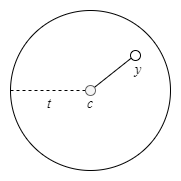
\includegraphics[scale=0.5]{figures/Diagrama_decodificacion_maxima_verosimilitud.png}
    \end{wrapfigure}

    $$y = c + e \in \mathbb{F}^n,$$

    donde $e$ denota al vector error.
    
    Esto satisface 

    $$d(c,y) = d(e,0) \leq t,$$

    y por lo tanto $c$ es el único elemento de $\mathcal{C}$ que se encuentra en una bola de radio $t$ alrededor de $y$. Un decodificador de máxima verosimilitud produce este elemento $c$, y así se obtiene el código correcto.
\end{proof}

\begin{definition}
    El \emph{peso Hamming} $\operatorname{wt}(\mathbf{x})$ de un vector $\mathbf{x} \in \mathbb{F}_q^n$ se define como el número de coordenadas no nulas en $\mathbf{x}$.
\end{definition}

\begin{exampleth}
    Sea $\mathbf{x} = 2001021 \in \mathbb{F}_3^7$ un vector, entonces su peso Hamming es $wt(\mathbf{x}) = 4$.
\end{exampleth}

El siguiente resultado nos muestra la relación entre la distancia y el peso.

\begin{theorem}
    Si $\mathbf{x}, \mathbf{y} \in \mathbb{F}_q^n$, entonces $\operatorname{d}(\mathbf{x},\mathbf{y}) = \operatorname{wt}(\mathbf{x}-\mathbf{y})$. Si $\mathcal{C}$ es un código lineal, entonces la distancia mínima $d$ coincide con el peso mínimo de las palabras código no nulas de $\mathcal{C}$.
\end{theorem}

\begin{proof}
    Sean $x,y \in \mathbb{F}_q^n$, por la definición de distancia de Hamming tenemos que $d(x,y) = wt(x-y)$. Se supone ahora que $C$ es un código lineal, luego para todo $x,y \in \mathcal{C}$, $x-y \in \mathcal{C}$, luego para cualquier par de elementos $x,y \in \mathcal{C}$, existe $z \in \mathcal{C}$ tal que $d(x,y) = wt(z) \geq wt(\mathcal{C})$, donde $wt(\mathcal{C})$ es el peso mínimo de $\mathcal{C}$. Por tanto, $d \geq wt(\mathcal{C})$. Por otro lado, para todo $x \in \mathcal{C}$, se tiene que $wt(x) = d(x,0)$. Como $\mathcal{C}$ es lineal, $0 \in \mathcal{C}$, luego $d(x,0) \geq d$. Entonces, $wt(\mathcal{C}) \geq d$. Se concluye que $wt(\mathcal{C}) = d$, como se quería.
\end{proof}

Como consecuencia de este teorema, para códigos lineales, la distancia mínima también se denomina \emph{peso mínimo} de un código. Si se conoce el peso mínimo $d$ de un $[n,k]$ código, se dice entonces que es un $[n,k,d]_q$ código.

En el artículo \cite{Vardy_1997} se ha demostrado que el problema de calcular la distancia mínima de un código lineal binario es NP-duro, y el problema de decisión correspondiente es NP-completo.

\begin{problemth}[Distancia mínima]
    \label{pr:min-dist}
    Dada una matriz binaria $H$ de dimensión $m \times n$ y un número entero $w > 0$. ¿Existe un vector no nulo $x \in \mathbb{F}_2^n$ de peso menor que $w$ tal que $Hw^T = 0$? 
\end{problemth}

El problema \ref{pr:min-dist} es un problema NP-completo. Veamos un esquema de la demostración de este resultado. Para ello, haremos uso de una transformación polinomial del problema de Decodificación de Máxima Verosimilitud al problema de Distancia Mínima.

\begin{problemth}[Decodificación de Máxima Verosimilitud]
    \label{pr:dmv}
    Dados una matriz binaria $H$ de dimensión $m \times n$, un vector $s \in \mathbb{F}_2^m$ y un número entero $w > 0$. ¿Existe un vector $x \in \mathbb{F}_2^n$ de peso menor o igual que $w$ tal que $Hx^t = s$?
\end{problemth}

El problema \ref{pr:dmv} es NP-completo y sigue siendo NP-completo bajo ciertas restricciones, luego reformularemos este problema como la versión de campo finito de Suma de Subconjuntos, un problema NP-completo conocido. Además, calcular la distancia mínima para la clase de códigos lineales sobre un cuerpo de característica 2 es NP-duro, y el problema de decisión correspondiente Distancia Mínima sobre $GF(2^m)$, abreviado $MD_{2^m}$, es NP-completo. Luego esta prueba se basa en una transformación polinomial de Decodificación de Máxima Verosimilitud a $MD_{2^m}$. Sin embargo, esto no prueba que Distancia Mínima sea NP-completo, ya que el posible conjunto de entradas a Distancia Mínima es un pequeño subconjunto del conjunto de posibles entradas a $MD_{2^m}$. Para ello, se construye una aplicación del código $\mathbb{C\#}$ sobre $GF(2^m)$ a un código binario $\mathbb{C}$, de tal forma que la distancia mínima de $\mathbb{C\#}$ puede determinarse a partir de la distancia mínima de $\mathbb{C}$. Dado que la longitud de $\mathbb{C}$ está acotada por la longitud de un polinomio de $\mathbb{C\#}$, y el mapeo en sí se puede lograr en tiempo polinomial, esto completa la prueba de la NP-completitud de Distancia Mínima.


\begin{definition}
    Sea $A_i$, también denotada por $A_i(\mathcal{C})$, el número de palabras código con peso $i$ en $\mathcal{C}$. Se dice que la lista $A_i$ para $0 \leq i \leq n$ es la distribución del peso o espectro del peso de $\mathcal{C}$.
\end{definition}

\section{Clasificación por isometría}

Como hemos visto, las propiedades de un código dependen principalmente de las distancias de Hamming entre sus palabras y entre palabras codificadas y no codificadas. Además, puede ser que un código pueda relacionarse con otro por medio de una aplicación que conserve las distancias de Hamming. De esta forma, podemos definir una relación de equivalencia entre dos códigos que preservan la distancia de Hamming.

Sean $C$ y $C'$ dos $[n,k]_q$ códigos, se dice que son de la \emph{misma cualidad} si existe una aplicación

$$\iota : F^n_q \rightarrow F^n_q$$

con $\iota(C) = C'$ que preserva la distancia de Hamming, es decir, 

$$d(w,w') = d(\iota (w), \iota(w')), \qquad \forall w,w' \in H(n,q).$$

Las aplicaciones con la propiedad anterior se llaman \emph{isometrías}.

\begin{definition}
    Dos códigos lineales $C, C' \subseteq H(n,q)$ se llaman \emph{isométricos} si existe una isometría de $H(n,q)$ que aplica $C$ sobre $C'$.
\end{definition}

Las permutaciones de las coordenadas son isometrías, que se denominan \emph{isometrías permutacionales}.

\begin{definition}
    Sea $S_n$ el grupo isométrico en el conjunto $X = n = \left\{ 0,..., n-1 \right\}$. Dos códigos lineales $C, C' \subseteq H(n,q)$ son isométricos permutacionalmente si existe una isometría permutacional de $H(n,q)$ que aplica $C$ sobre $C'$. Esto es, hay una permutación $\pi$ en el grupo simétrico $S_n$ tal que 

    $$ C' = \pi (C) = \left\{ \pi(c) : c \in C \right\}, \quad \text{ and } \quad d(c, \tilde{c}) = d(\pi(c), \pi(\tilde{c})), \qquad \forall c,\tilde{c} \in C,$$ 

    donde
    
    $$\pi(c) = \pi(c_0,...,c_{n-1}) := \left( c_{\pi ^{-1} (0)}, ..., c_{\pi ^{-1} (n-1)} \right)$$
\end{definition}

\section{Algoritmo para el cálculo de la distancia}

Como hemos visto, la distancia mínima es importante en un código lineal. Sin embargo, calcular este parámetro para un código dado puede resultar laborioso. A continuación presentaremos el algoritmo de BZ para el cálculo de la distancia, que tiene eficiencia exponencial \cite[Sección 1.8]{Wassermann_2006}. Este algoritmo destaca por ser el algoritmo más rápido para calcular la distancia mínima de un código lineal. En particular, si el código es binario se considera eficaz.

\begin{Ualgorithm}[H]
    \DontPrintSemicolon
    \KwIn{matriz generadora $G_1 = (I_k | A_1)$ de $\mathcal{C}$}
    \KwOut{distancia mínima $\bar{d}_i$}
    $m \longleftarrow 2$\;
    $k_1 \longleftarrow k$\;
    \While{rank $(A_m) \neq 0$}{
        Aplicar la eliminación de Gauss y posibles permutaciones de las columnas de la matriz $A_{m-1}$ desde $G_{m-1} = \left( \begin{array}{c|c} A_{m-1}' & \begin{array}{c|c} I_{k_{m-1}} & A_{m-1} \\ \hline  0 & 0 \end{array} \end{array} \right)$ para obtener la matriz generadora $G_{m} = \left( \begin{array}{c|c}  A_{m}' & \begin{array}{c|c}   I_{k_{m}} & A_{m} \\  \hline 0 & 0  \end{array}  \end{array} \right)$\;
    }
    $C_0 \longleftarrow \left\lbrace 0 \right\rbrace$\;
    $i \longleftarrow 0$\;
    \While{$\bar{d}_i > \underline{d}_i$}{
        $i \longleftarrow i + 1$\;
        $C_i \longleftarrow C_{i-1} \cup \bigcup_{j=1}^m \left\lbrace v \cdot G_j : v \in \mathbb{F}_q^k, \; wt(v) = i \right\rbrace$\;
        $\bar{d}_i \longleftarrow \min \left\{ wt(c) : c \in C_i, \; c \neq 0 \right\}$\;
        $\underline{d}_i \longleftarrow \sum_{\substack{j=1\\ k-k_j \leq i}}^m \left( (i+1)-(k-k_j) \right)$\;
    }
    \caption{Algoritmo de Brouwer-Zimmermann: cálculo de la distancia mínima de un $[n,k]$ código lineal $\mathcal{C}$.}
\end{Ualgorithm}

Veamos, en efecto, que este algoritmo determina la distancia mínima. Consideramos $\mathcal{C}$ un $[n, k]_q$ código lineal y $G$ una matriz generadora. Como el código es lineal, existen matrices $M \in M_n(q)$ y $B \in GL_k(q)$ tales que $B \cdot G \cdot M^T$ es una matriz generadora en forma estándar. De hecho, usando el método de Gauss, podemos obtener una matriz generadora en forma estándar mediante operaciones elementales en las filas y permutaciones de las columnas. En este caso para realizar las operaciones elementales en las filas multiplicaremos desde la izquierda por una matriz $B_1 \in GL_k(q)$, y para permutar las columnas multiplicaremos desde la derecha por la traspuesta de una matriz de permutaciones $M_{\pi_1}$, de tal forma que

$$G_1 := B_1 \cdot G \cdot M_{\pi_1}^T = \left( I_{k_1} | A_1 \right),$$

donde $k_1 = k$.

Ahora que tenemos la matriz generadora en forma estándar, necesitaremos tranformarla de nuevo. Si $A_1$ no es una matriz nula ni vacía, su rango será $k_2$ con $0 < k_2 \leq k_1$. Aplicando la eliminación de Gauss, podemos obtener $k_2$ vectores unitarios diferentes en las $n - k_1$ columnas. Esto es, podemos multiplicar a $G_1$ desde la izquierda por una matriz $B_2 \in GL_k(q)$ y desde la derecha por la traspuesta de una matriz de permutaciones $M_{\pi_2}$ con $\pi_2(j) = j$ para $0 \leq j < k_1$, obteniendo

$$G_2 := B_2 \cdot G_1 \cdot M_{\pi_2}^T = \left( \begin{array}{c|c} A_{2}' & \begin{array}{c|c} I_{k_{2}} & A_{2} \\ \hline  0 & 0 \end{array} \end{array} \right).$$

De esta forma, obtenemos que la matriz $A_2'$ es una matriz $k \times k_1$ y la matriz $A_2$ es una matriz $k_2 \times (n - k_1 - k_2)$. Los ceros indican las matrices nulas.

Una vez que tenemos la matriz generadora de esta forma, realizaremos un procedimiento iterativo aplicando la eliminación de Gauss y posibles permutaciones de las columnas de la matriz $A_2$ hasta que su rango sea 0. Esto es, sea $i \geq 2$, la matriz $A_i$ tiene rango $k_{i+1}$ con $0 < k_{i+1} \leq k_i$. En cada iteración, obtendremos matrices regulares $B_{i+1} \in GL_k(q)$, matrices de permutación $M_{\pi+1} \in M_n(q)$ con $\pi_{i+1}(j) = j$ para $0 \leq j < k_1 + \cdots + k_i$ y matrices generadoras

$$G_{i+1} := B_{i+1} \cdot G_i \cdot M_{\pi_{i+1}}^T = \left( \begin{array}{c|c} A_{i+1}' & \begin{array}{c|c} I_{k_{i+1}} & A_{i+1} \\ \hline  0 & 0 \end{array} \end{array} \right),$$

donde $A_{i+1}'$ es una matriz $k \times (k_1 + \cdots + k_i)$ y $A_{i+1}$ es una matriz $k_{i+1} \times (n - k_1 - \cdots - k_{i+1})$. Repitiendo este procedimiento, finalmente obtendremos una matriz generadora $G_m$ tal que 

$$G_{m} = B_m \cdot G_{m-1} \cdot M_{\pi_m}^T = \left( \begin{array}{c|c}  A_{m}' & \begin{array}{c|c}   I_{k_{m}} & A_{m} \\  \hline 0 & 0  \end{array}  \end{array} \right),$$

donde $A_m$ es una matriz vacía (que significa que no tiene columnas) o es una matriz nula. Entonces, $k_1 + \cdots + k_m \leq n$ y $A_m$ tiene $n - k_1 - \cdots - k_m$ columnas. En consecuencia, la matriz generadora $G_m$ tiene $n - k_1 - \cdots - k_m$ columnas nulas y por lo cual todos los elementos del código generado por $G_m$ tiene peso menor que $k_1 + \cdots + k_m$.

Definimos para $1 \leq i \leq k$ los siguientes conjuntos:

$$C_i := \bigcup_{j=1}^m \left\{ v \cdot G_j : v \in \mathbb{F}_q^k, \; wt(v) \leq i \right\}$$

Claramente, estos conjuntos forman una cadena ascendente

$$C_1 \subseteq \cdots \subseteq C_k,$$

y por lo tanto los pesos mínimos

$$\bar{d}_i := \min \left\{ wt(c) : c \in C_i, \; c \neq 0 \right\}$$

forman una secuencia decreciente

$$\bar{d}_1 \geq \cdots \geq \bar{d}_k = dist(C).$$

En la mayoría de los casos, no será necesario calcular todos estos valores. En efecto, primero calcularemos $\bar{d}_1$. Después, si $\bar{d}_i$ ya ha sido calculada para algún $i \geq 1$, lo compararemos con $\underline{d}_i$, que es un límite inferior para el peso de los elementos en $C \setminus C_i$. Si $\bar{d}_i \leq \underline{d}_i$, hemos terminado. Si no, repetiremos el mismo proceso para $\bar{d}_{i+1}$.

Para calcular los límites inferiores para los pesos en los complementos $C \setminus C_i$, elegimos un elemento $c \in C \setminus C_i$. Como $c \notin C_i$, entonces existe, para cada $j$, un vector $v^{(j)} \in \mathbb{F}_q^k$ tal que

$$c = v^{(j)} \cdot G_j, \quad 1 \leq j \leq m, \; \text{ y } \; wt(v^{(j)}) \geq i + 1.$$

Para estimar el peso de $c$, nos basaremos en los distintos lugares de información en $G_i$, es decir, las columnas que contienen la matriz identidad $I_{k_j}$. Estas son las columnas de índice $r$ para $k_i + \cdots + k_{j-1} \leq r < k_1 + \cdots + k_j$. Nos interesan las $k_j$ coordenadas $c_r$ de $c = v^{(j)} \cdot G_j$ correspondientes a estas $k_j$ columnas. Como $v^{(j)}$ tiene longitud $k$, estas entradas de $c$ contribuyen al menos el valor de $i + 1 - (k - k_j)$ al peso de $c$. Además, como los conjuntos son disjuntos, para diferentes $j$, tenemos que 

$$wt(c) \geq \sum_{j=1}^m \left( i + 1 - (k - k_j) \right).$$

Restringiendo esta suma a sumandos positivos, obtenemos el límite inferior

$$wt(c) \geq \sum_{j \; : \: k - k_j \leq i} \left( i + 1 - (k - k_j) \right) =: \underline{d}_i.$$

La secuencia de estos límites es incremental, pues el primer sumando es $i + 1$:

$$2 \leq \underline{d}_1 < \cdots < \underline{d}_k.$$

Además,

$$\underline{d}_k = m + \sum_{j=1}^m k_j.$$

Finalmente, como $wt(c) \leq k_1 + \cdots + k_m$ para todo $c \in C$, existe un índice $i_0$ tal que

$$\bar{d}_{i_0} \leq \underline{d}_{i_0}.$$

Para este $i_0$ se cumple que

$$\bar{d}_{i_0} := \min \left\{ wt(c) : c \in C_{i_0}, \; c \neq 0 \right\},$$

y se sigue cumpliendo que 

$$\underline{d}_{i_0} \leq \min \left\{ wt(c) : c \in C \setminus C_{i_0} \right\}.$$

Por lo que

$$\bar{d}_{i_0} = dist(C),$$

y la palabra código de peso $dist(C)$ se encuentra en $C_{i_0}$.

\begin{exampleth}
    Consideramos el $[7, 3]$ código binario $\mathcal{C}$ con matriz generadora 

    \[
        G_1 = \left( 
            \begin{array}{ccc|cccc}
                1 & 0 & 0 & 1 & 0 & 1 & 1 \\ 
                0 & 1 & 0 & 1 & 1 & 0 & 1 \\ 
                0 & 0 & 1 & 0 & 1 & 1 & 1 \\ 
            \end{array}
            \right) .
    \]

    Aplicaremos el algoritmo de BZ para calcular la distancia mínima de este código.

    Observamos que la matriz generadora $G_1$ ya está en forma estándar y su conjunto de información es $\{ 0,1,2 \}$. Luego lo primero que haremos será aplicar el método de Gauss y permutaciones de las columnas para transformar esta matriz generadora en una matriz generadora de la forma

    $$\left( \begin{array}{c|c} A_{2}' & \begin{array}{c|c} I_{k_{2}} & A_{2} \\ \hline  0 & 0 \end{array} \end{array} \right),$$

    para alguna matriz $A_2'$ de dimensión $3 \times k_1$ y alguna matriz $A_2$ de dimensión $k_2 \times (7 - k_1 - k_2)$. En nuestro caso, tenemos que

    \[
        G_2 := \left( 
            \begin{array}{ccc|ccc|c}
                0 & 1 & 1 & 1 & 0 & 0 & 1 \\ 
                1 & 1 & 0 & 0 & 1 & 0 & 1 \\ 
                1 & 1 & 1 & 0 & 0 & 1 & 0 \\ 
            \end{array}
            \right) .
    \]

    Esta matriz generadora tiene conjunto de información $\{3,4,5\}$. El siguiente paso será realizar de nuevo la eliminación de Gauss y posibles permutaciones de las columnas de la matriz $A_2$ hasta que su rango sea $0$. El algoritmo nos dará la siguiente matriz generadora

    \[
        G_3 := \left( 
            \begin{array}{cccccc|c}
                0 & 1 & 1 & 1 & 0 & 0 & 1 \\ 
                1 & 0 & 1 & 1 & 1 & 0 & 0 \\ 
                1 & 1 & 1 & 0 & 0 & 1 & 0 \\ 
            \end{array}
            \right) .
    \]

    Esta matriz generadora tiene conjunto de información $\{6\}$. El conjunto $C_1$ está formado por las filas de las tres matrices generadoras $G_1$, $G_2$ y $G_3$. Ahora, calculamos el peso de cada uno de ellos, esto es, el número de coordenadas no nulas de cada elemento y obtenemos que todos tienen peso $4$, por lo que $\bar{d}_1 = 4$. El límite inferior del peso mínimo de los vectores que no pertenecen a $C_1$ es $\underline{d}_1 = 1 + 1 - (3-3) + 1 + 1 - (3-3) = 4$. Concluimos que $d = \bar{d}_1 = 4$ es la mínima distancia de $C$.
\end{exampleth}

